\subsection{About ARFC}
\begin{frame}
  \frametitle{Advanced Reactors and Fuel Cycles group (PI: Kathryn Huff)}
               \begin{figure}[t]
                \vspace*{-0.25in}
                \hspace*{-0.35in}
                
\includegraphics[height=0.63\textwidth]{./images/arfc1.png}
                \caption{Current Advanced Reactors and Fuel Cycles Group researchers.}
               \end{figure}            
\end{frame}

\begin{frame}
  \frametitle{Advanced Reactors and Fuel Cycles group (PI: Kathryn Huff)}
               \begin{figure}[t]
                
\includegraphics[height=0.33\textwidth]{./images/arfc_past.png}
                \caption{Past ARFC Group members who contributed to this work.}
               \end{figure}            
\end{frame}


\subsection{Molten salt reactors}
\begin{frame}
  \frametitle{Molten Salt Reactor Types}
                  \vspace*{-0.1in}
              \begin{block}{Stationary Fuel}
               \begin{enumerate}
                \item Graphite block with TRISO fuel, clean salt works as coolant (e.g. TMSR-SF1, FHR-DR)
                \item Plate Fuel: hexagonal fuel assembly is similar in shape to a typical sodium-cooled reactor
                        % Not sure what FIRM is.
                %\item Fuel Inside Radial Moderator (FIRM)
                        % While it doesn't leave the reactor, doesn't 
                        % the fuel in the moltex reactor move up and down?
                        % If the fluid is free to naturally circulate inside 
                        % the rod, it likely happens on 
                        % timescales that I do not think we can ignore from a 
                        % kinetics perspective. 
                %\item Liquid fuel salt inside fuel rods cooled by clean salt (e.g. Moltex Stable Salt Reactor)
               \end{enumerate}
               \end{block}
               
               \begin{block}{Mobile Fuel}
               \begin{enumerate}
                \item Mobile solid fuel elements (e.g. pebbles) cooled by clean salt (e.g. PB-FHR)
                \item Non-circulating liquid fuel salt (e.g. TerraPower MCFR) 
                \item \textbf{Circulating fuel salt} which also works as coolant (e.g. \gls{MSRE}, \gls{MSBR}, TAP MSR)
               \end{enumerate}
               \end{block}
\end{frame}

\begin{frame}
  \frametitle{Stationary and Mobile Solid fuel}
        \vspace*{-0.1in}
               \begin{figure}[t]
			\hspace*{-0.35in}
                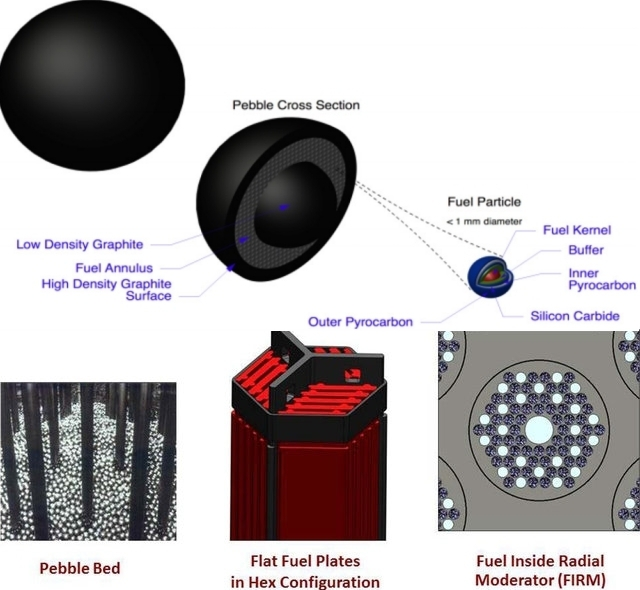
\includegraphics[height=0.63\textwidth]{./images/solid_fuel.jpg}
                \caption{TRISO fuel particle (top) and FHR fuel designs (bottom). Source \cite{forsberg_basis_2016-1}.}
             \end{figure}   
\end{frame}

\begin{frame}
  \frametitle{Mobile, Non-Circulating, Liquid Fuel}
               \begin{figure}[t]
                \vspace*{-0.1in}
			\hspace*{-0.35in}
                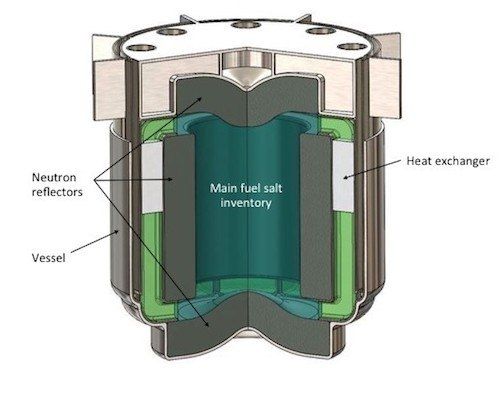
\includegraphics[height=0.6\textwidth]{./images/mcfr-crossection.jpg}
                \caption{The TerraPower MCFR is an example of reactor design with \textbf{liquid, mobile, non-circulating} chloride salt fuel. Source \cite{doene_southern_2018}.}
             \end{figure}   
  
\end{frame}

\begin{frame}
  \frametitle{Mobile, Circulating, Liquid Fuel}
               \begin{figure}[t]
                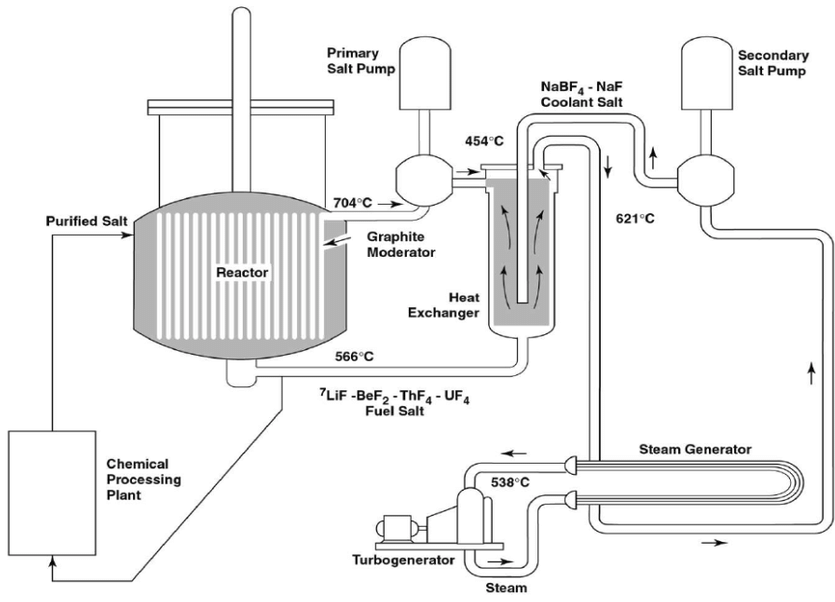
\includegraphics[height=0.58\textwidth]{./images/msbr_scheme.png}
                \caption{The \gls{MSBR} is an example of reactor design with \textbf{liquid, mobile, circulating} fluoride salt fuel \cite{rosenthal_molten-salt_1970}.}
             \end{figure}   
  
\end{frame}

\subsection{Motivation}
\begin{frame}
  \frametitle{Why Molten Salt Reactors with circulating fuel?}
              \begin{block}{Main advantages of liquid-fueled \glspl{MSR} \cite{elsheikh_safety_2013}}
               \begin{enumerate}
                \item High coolant temperature (600-750$^{\circ}$C)
                \item Fuel diversity ($^{235}$U, $^{233}$U, Thorium, U/Pu)
                \item Increased inherent safety
                \item High fuel utilization $\Rightarrow$ less nuclear waste generated
                \item Online reprocessing and refueling
                \item Thermal/epithermal (\gls{MSBR}) or fast spectrum (\gls{MSFR})
                \item Can produce more fissile material than it consumes (breeder)
                \item Nuclear Spent Fuel Transmuter (e.g. REBUS-3700 \cite{mourogov_potentialities_2006-1}, MOSART \cite{ignatiev_molten_2014}) 
               \end{enumerate}
               \end{block}

\end{frame}

\begin{frame}
  \frametitle{Challenges in \gls{MSR} Simulation}
                  \vspace*{-0.05in}
               \begin{enumerate}
                \item Contemporary burnup codes cannot treat fuel movement
                \item Neutron precursor location is hard to estimate
                \item Operational and safety parameters change during reactor operation
                \item Power generation strongly depends on fuel temperature and vica versa
               \end{enumerate}

           \begin{figure}[t]
                \vspace*{-0.05in}
			\hspace*{-0.2in}
                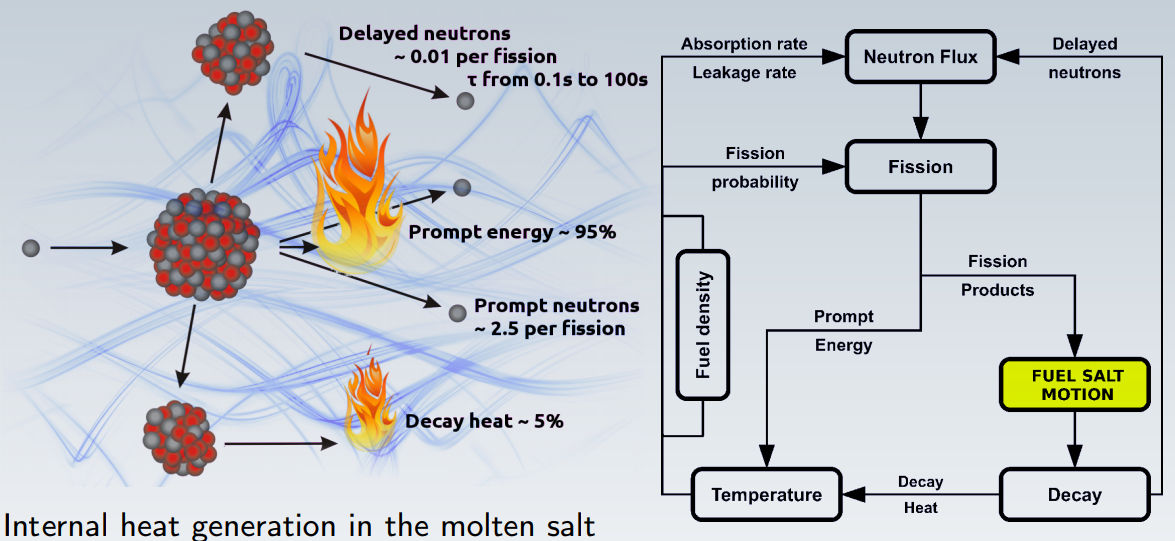
\includegraphics[height=0.47\textwidth]{./images/coupled_physics.png}
		\vspace*{-0.05in}
		\caption{Challenges in simulating \glspl{MSR} (Image courtesy of Manuele Aufiero,2012).}
     	 \end{figure}               
\end{frame}

\begin{frame}
  \frametitle{Research objectives}
                  \vspace*{-0.1in}

              \begin{block}{Multiphysics simulation of \gls{MSR} (Moltres/MOOSE)\cite{lindsay_introduction_2018}}
               \begin{enumerate}
                \item Demonstrate steady-state and transient coupling of neutron fluxes, precursor drift, and thermal-hydraulics
                \item Implement advective movement of delayed neutron precursors
                \item Demonstrate capabilities with 2D axisymmetric and 3D mesh
                \item Simple transients: change of flow and moderator movement
               \end{enumerate}
               \end{block}


              
\end{frame}
